\documentclass[11pt]{article}
%\usepackage{psfig}
\usepackage{graphicx}
\usepackage{enumitem}
\usepackage{amsmath,amssymb,amsthm,listings,hyperref}
\usepackage{tikz}
\usepackage{latexsym}
\usepackage{amsfonts}

\title{CS 4641 Project 3 Report}
\author{HU Heng}
\date{March 23, 2019}
\begin{document}
\maketitle
\section{Overview}
This report is for CS 4641 Machine Learning project 3 Unsupervised Learning. In the following pages, you will see clustering algorithms including Expectation Maximization and K means and dimensionality reduction algorithms including PCA, ICA, Randomized Projection and Feature Selection. I will apply the algorithms on the dataset I used in my project 1 and show the results by some figures and analysis.\\

\section{Datasets}
The datasets I choose are wine dataset and adult dataset which are used in my project 1.
\subsection{Adult Dataset}
Adult dataset is extracted from the 1994 Census database. There are 14 attributes and the result is whether the income is greater than \$50k or not. It is a binary classification problem and there are 48842 instances in total. 
\subsection{Wine Dataset}
Wine data are the results of a chemical analysis of wines grown in the same region in Italy but derived from three different cultivars. There are 13 dimensions and three possible classes. There are 178 instances in total. 

%\begin{figure}
%  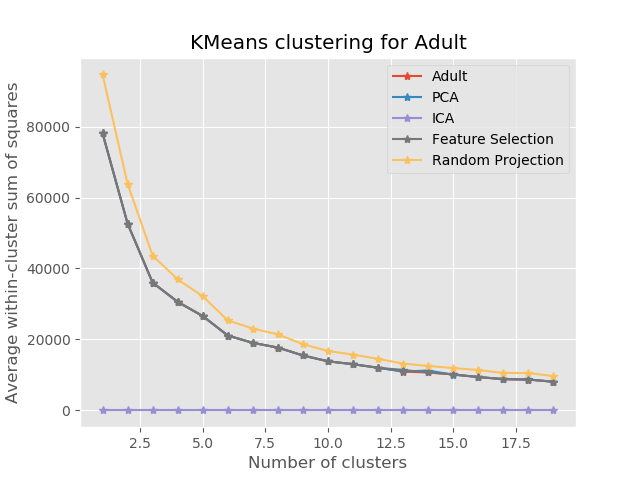
\includegraphics[width=\linewidth]{../figures/cluster_kmeans_adult.png}
%  \caption{A boat.}
%  \label{fig:cluster_kmeans_adult}
%\end{figure}
\section{Clustering}
\subsection{K means}
To select a good K, I would like to run K means algorithm multiple times on the two datasets with different K and see the results. K means will start with random cluster centers that have components on each of the given dimensions of the data. Using a distance function, it distributes each instance to the closest cluster center and in the end, takes the mean of the clusters to calculate the new cluster center and restarts the distribution process. It loops until the centers’ coordinates on the hyper-dimensions stops changing. I will use sum of squared error to justify the ``goodness'' of the result. Fig.\ref{Fig:cluster_kmeans_adult} is the result for adult dataset and Fig.\ref{Fig:cluster_kmeans_wine} is the result for wine dataset. It can be predicted that the more cluster we get, the better the result. The trade off is that we are making the data more complicated. \\
\\
These two figures also contains the curve for doing dimension reduction first and apply K menas algorithm on reduced data. Here the result is very close and I can hardly find any difference for wine dataset. For adult dataset, the difference is also very small.\\
\\
\begin{figure}[!htb]
   \begin{minipage}{0.5\textwidth}
     \centering
     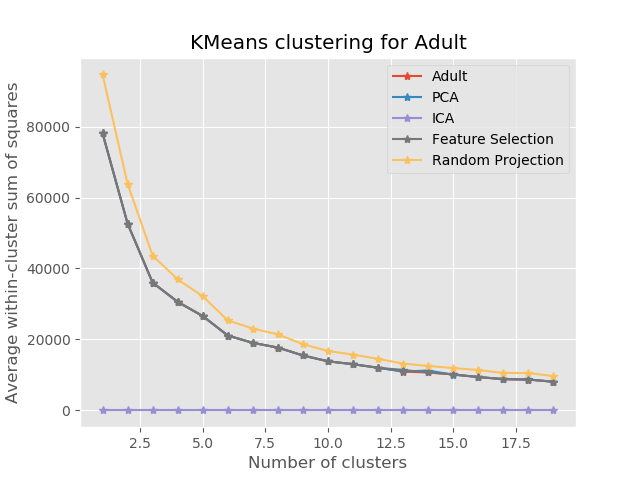
\includegraphics[width=1.2\linewidth]{../figures/cluster_kmeans_adult.png}
     \caption{Adult}\label{Fig:cluster_kmeans_adult}
   \end{minipage}\hfill
   \begin{minipage}{0.5\textwidth}
     \centering
     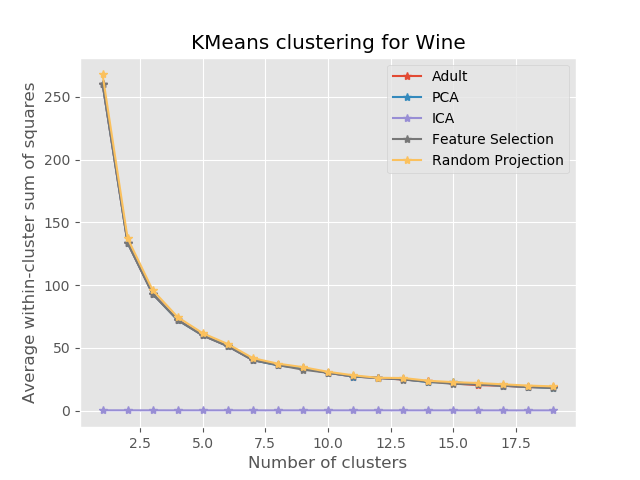
\includegraphics[width=1.2\linewidth]{../figures/cluster_kmeans_wine.png}
     \caption{Wine}\label{Fig:cluster_kmeans_wine}
   \end{minipage}
\end{figure}

\subsection{Expectation Maximization}
Expectation Maximization (EM) is another clustering algorithm that is similar to K means clustering. EM is a more general algorithm and K means is a specific version of it. Instead of directly place the data point into a certain center, EM will assign data points to cluster centers with different probabilities. Thus an instance can be belongs to multiple clusters with certain probability. The result of EM is again several cluster centers that cover different areas of all data points and the list of all the instances with their cluster that probably include them. Log likelihood describes how the instance is related to the cluster center and the result is shown in Fig.\ref{Fig:cluster_em_ll_adult} for adult dataset and Fig.\ref{Fig:cluster_em_ll_wine} for wine dataset. \\
\\
These two figures also contains the curve for doing dimension reduction first and apply EM algorithm on reduced data. It is clear that log likelihood goes up as number of clusters increases. This is what I expect because large log likelihood means the data points is closer to a certain cluster center. Increase the number of clusters will increase log likelihood trivially. Another observation is that apply ICA before clustering will produce much higher log likelihood result, which is because ICA is going to find the independent vectors. Treat clusters as linearly independent vectors and log likelihood describes the data points in each vectors.  Fig.\ref{Fig:cluster_em_aic_adult} and Fig.\ref{Fig:cluster_em_aic_wine} shows the AIC value for two datasets. Fig.\ref{Fig:cluster_em_bic_adult} and Fig.\ref{Fig:cluster_em_bic_wine} shows the BIC value for two datasets.
\begin{figure}[!htb]
   \begin{minipage}{0.5\textwidth}
     \centering
     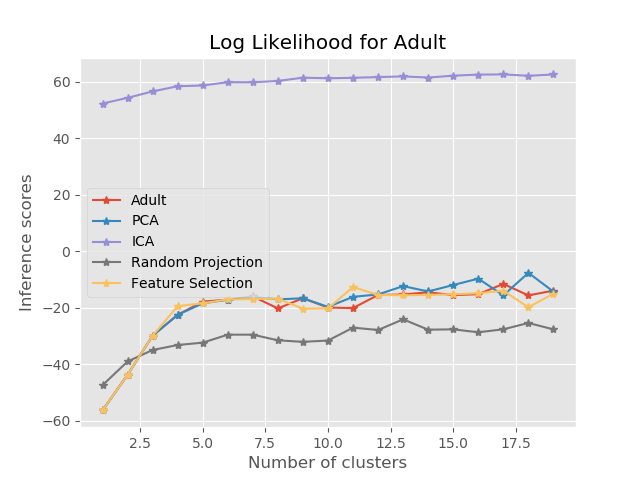
\includegraphics[width=1.2\linewidth]{../figures/cluster_em_ll_adult.png}
     \caption{Adult Log Likelihood}\label{Fig:cluster_em_ll_adult}
   \end{minipage}\hfill
   \begin{minipage}{0.5\textwidth}
     \centering
     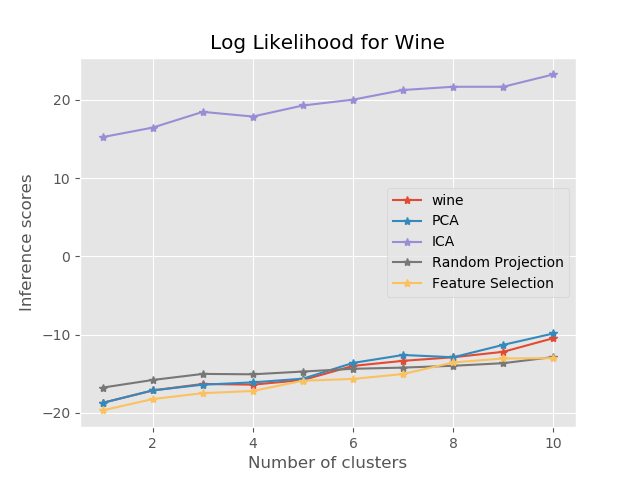
\includegraphics[width=1.2\linewidth]{../figures/cluster_em_ll_wine.png}
  \caption{Wine Log Likelihood}
  \label{Fig:cluster_em_ll_wine}
   \end{minipage}
\end{figure}
\begin{figure}[!htb]
   \begin{minipage}{0.5\textwidth}
     \centering
     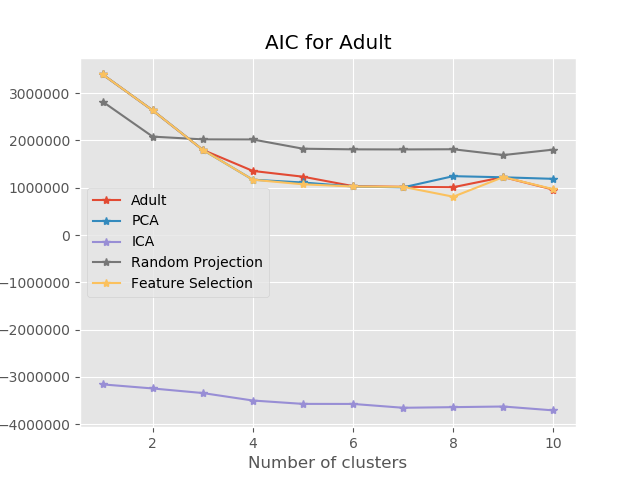
\includegraphics[width=1.2\linewidth]{../figures/cluster_em_aic_adult.png}
     \caption{Adult AIC}\label{Fig:cluster_em_aic_adult}
   \end{minipage}\hfill
   \begin{minipage}{0.5\textwidth}
     \centering
     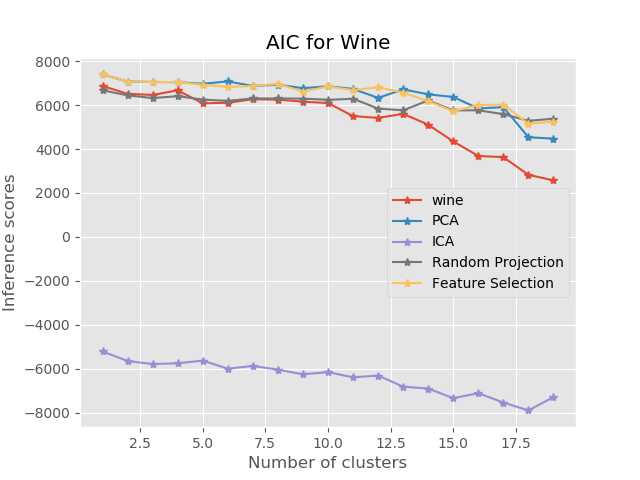
\includegraphics[width=1.2\linewidth]{../figures/cluster_em_aic_wine.png}
  \caption{Wine AIC}
  \label{Fig:cluster_em_aic_wine}
   \end{minipage}
\end{figure}
\begin{figure}[!htb]
   \begin{minipage}{0.5\textwidth}
     \centering
     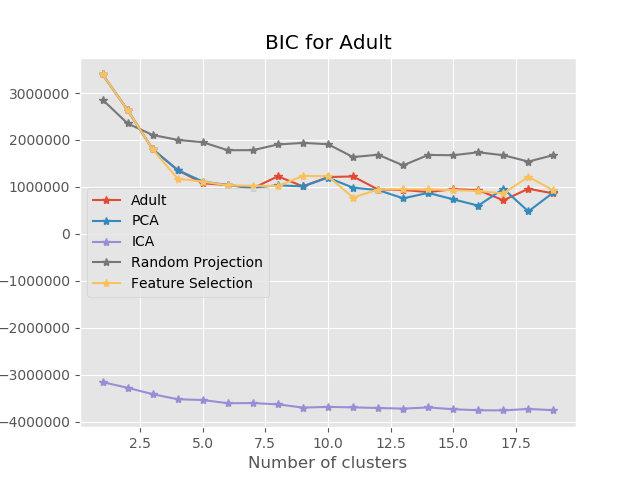
\includegraphics[width=1.2\linewidth]{../figures/cluster_em_bic_adult.png}
     \caption{Adult BIC}\label{Fig:cluster_em_bic_adult}
   \end{minipage}\hfill
   \begin{minipage}{0.5\textwidth}
     \centering
     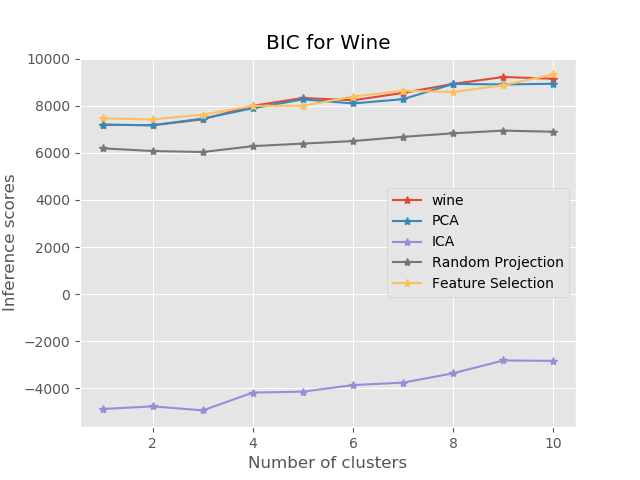
\includegraphics[width=1.2\linewidth]{../figures/cluster_em_bic_wine.png}
  \caption{Wine BIC}
  \label{Fig:cluster_em_bic_wine}
   \end{minipage}
\end{figure}
\subsection{Data After Clustering}
Another interesting question is what does my data look like after clustering. To have a better idea, I use the wine dataset and plot the result after clustering using K means algorithm. The cluster centers are the big blue points. Fig.\ref{Fig:km_wine_3} uses 3 clusters and Fig.\ref{Fig:km_wine_5} uses 5 clusters. From the figures, we can see clearly that some parts of the data points are aggregated together with a ``center''. The data points are almost equally separated. To describe it in another way, the data are ``clustered'' into different parts to minimize the sum of square error between each point and the center point.
\begin{figure}[!htb]
   \begin{minipage}{0.5\textwidth}
     \centering
     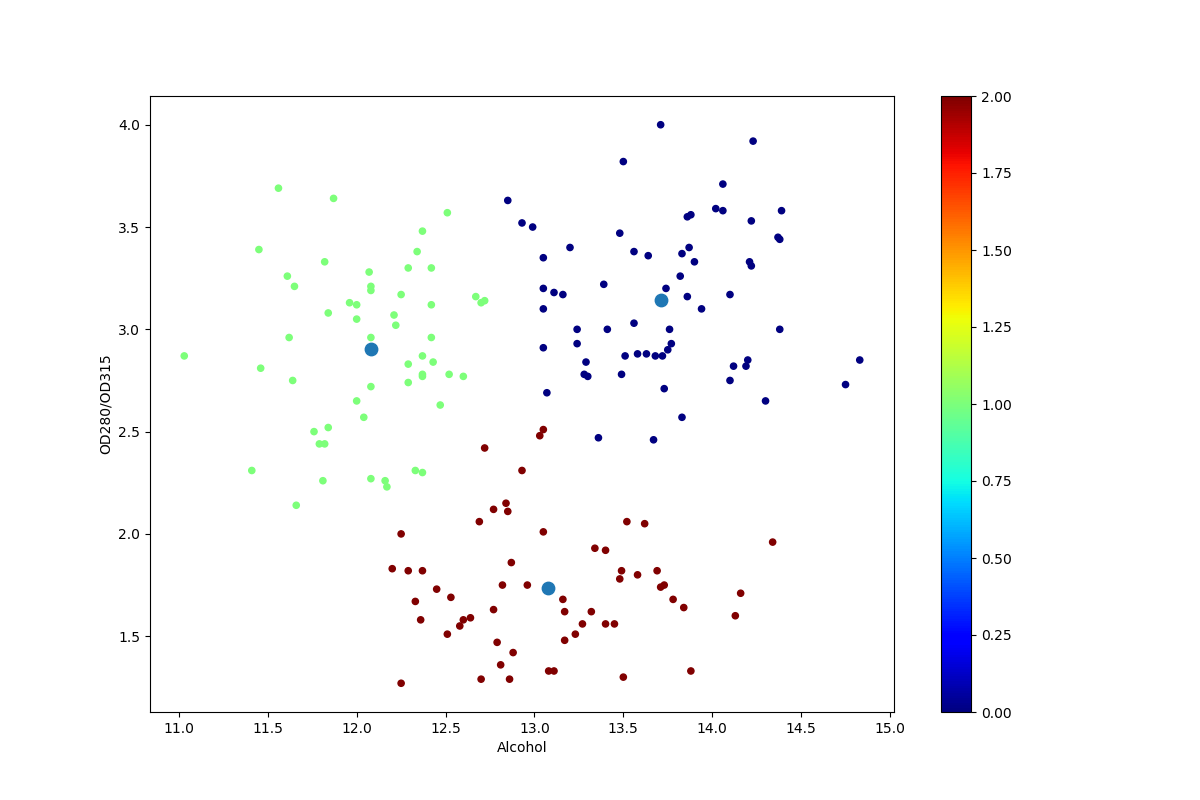
\includegraphics[width=1.2\linewidth]{../figures/km_wine_3.png}
     \caption{3 clusters}\label{Fig:km_wine_3}
   \end{minipage}\hfill
   \begin{minipage}{0.5\textwidth}
     \centering
     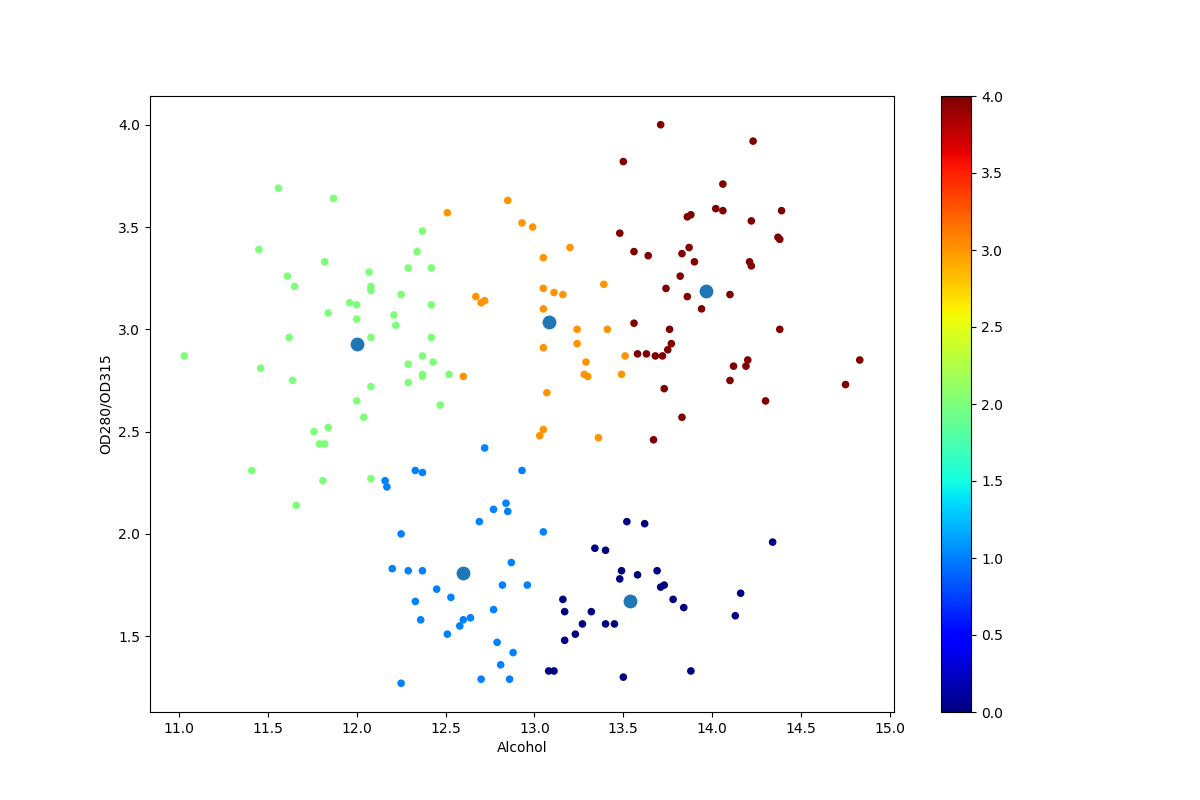
\includegraphics[width=1.2\linewidth]{../figures/km_wine_5.png}
     \caption{5 clusters}\label{Fig:km_wine_5}
   \end{minipage}
\end{figure}

\section{Dimension Reduction}
\subsection{PCA}
PCA will reduce the trends in the data to eigenvectors that represent the major correlations of a given dataset. It tries to find the eigenvector that has the highest variance in order to account for the maximum variability in the data to cover as much instances as possible. Fig.\ref{Fig:pca_wine} shows the wine dataset after applying PCA. There are 13 variables originally and these are shown in the figure by red lines. Points with same colors are actually belongs to the same class. It is clear that data points are well separated. More generally, the process of dimension reduction is to generate a map function and map the raw data from high dimensional space to low dimensional space. Data points from same class will be ``closer'' after dimensional reduction.
\begin{figure}
 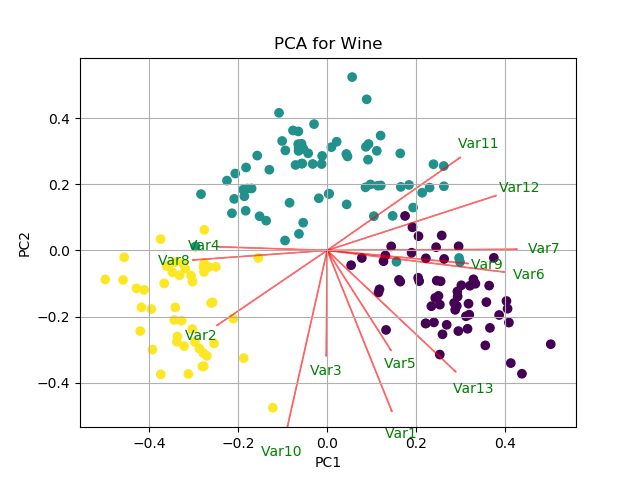
\includegraphics[width=\linewidth]{../figures/pca_wine.png}
 \caption{Data after PCA}
 \label{Fig:pca_wine}
\end{figure}
\subsection{ICA}
ICA is another dimension reduction algorithm that tries to reduce the data into linearly independent vectors. The difference between ICA and PCA is that ICA is going to find the linearly independent vectors while PCA is going to find orthogonal directions in the raw feature space that correspond to directions accounting for maximum variance. 
\subsection{Random Projection}
Random projections is another dimension reduction algorithm that works different with PCA and ICA. It is a simple and computationally efficient way to reduce the dimensionality of the data by trading a controlled amount of accuracy (as additional variance) for faster processing times and smaller model sizes. In my experiment, I use Gaussian Random Projection.
\subsection{Feature Selection}
\begin{table}[h!]
  \begin{center}
    \caption{Performance of Algorithms}
    \label{tab:wine_fs}
    \begin{tabular}{c|c|c}
      \textbf{Threshold} & \textbf{Accuracy} & \textbf{Training Time}\\
      \hline
      0.025 & 39.88\% & 0.01097 \\
      0.050 & 28.08\% & 0.01795\\
      0.075 & 39.88\% & 0.01097\\
      0.100 & 39.88\% & 0.00897\\
      0.125 & 49.43\% & 0.01795\\
      0.150 & 26.96\% & 0.01396\\
      0.175 & 33.14\% & 0.01097\\
      0.200 & 26.96\% & 0.01097\\
      0.225 & 39.88\% & 0.00997\\
      0.250 & 39.88\% & 0.01296\\
      0.275 & 39.88\% & 0.01197\\
      0.300 & 33.14\% & 0.01096\\
    \end{tabular}
  \end{center}
\end{table}
I use variance threshold algorithm as the last dimension reduction algorithm. It is very simple and easy to understand. It will look over the features and if the variance of a feature is lower than threshold, the feature will be removed. I use this feature selection algorithm to reduce dimension and feed the data to neural network. The different selection of threshold will influence the accuracy, as shown in Table.\ref{tab:wine_fs}. I may conclude that very low threshold cannot give good accuracy because there still are some useless information or noise. Very large threshold also cannot give good accuracy since it is ``over-reduce''(like overfit) and remove too much useful information. From the experiments, 0.125 is a good threshold for wine dataset.

\section{Rerun Neural Network on Wine Dataset}
\subsection{Apply Dimension Reduction Algorithm}
\begin{figure}[!htb]
   \begin{minipage}{0.5\textwidth}
     \centering
     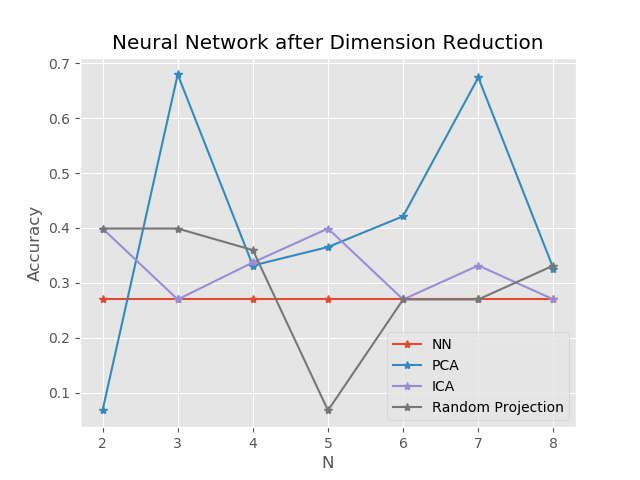
\includegraphics[width=1.2\linewidth]{../figures/wine_nn_dr.png}
     \caption{Accuracy}\label{Fig:wine_nn_dr}
   \end{minipage}\hfill
   \begin{minipage}{0.5\textwidth}
     \centering
     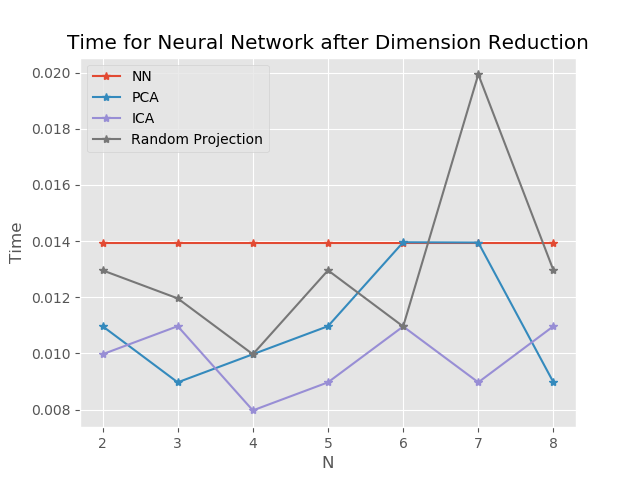
\includegraphics[width=1.2\linewidth]{../figures/wine_nn_dr_time.png}
     \caption{Time}\label{Fig:wine_nn_dr_time}
   \end{minipage}
\end{figure}

Fig.\ref{Fig:wine_nn_dr} shows the accuracy of neural networks trained by data that is preprocessed by different dimension reduction algorithms. Fig.\ref{Fig:wine_nn_dr_time} shows the corresponding training time. The x-axis is different selection of N. From the figure, the training time is reduced slightly and the performance is better than the neural network trained by original data. By reduction the dimensions, the training time is slightly reduced since there is less computation. Table.\ref{tab:wine_fs} shows the performance of using different threshold for feature selection algorithm. Similarly, the accuracy is higher and the training time is reduced. The accuracy increases because the data in high dimensional space may contain noise or useless information. After dimension reduction, the data contain less noise or useless information, thus increasing the accuracy.
\subsection{Apply Clustering Algotithm}
\begin{figure}[!htb]
   \begin{minipage}{0.5\textwidth}
     \centering
     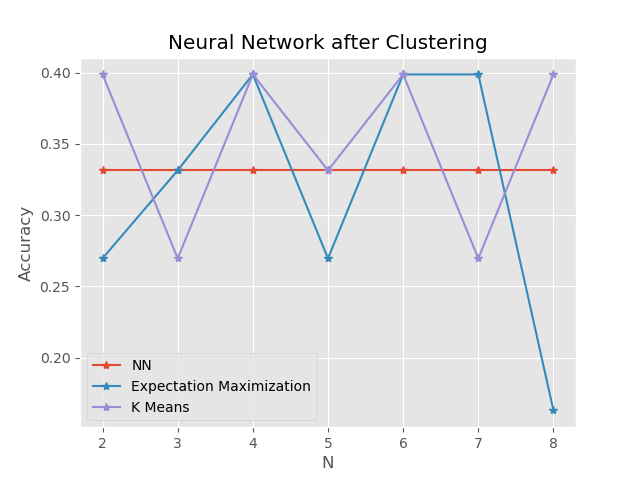
\includegraphics[width=1.2\linewidth]{../figures/wine_nn_cluster.png}
     \caption{Accuracy}\label{Fig:wine_nn_cluster}
   \end{minipage}\hfill
   \begin{minipage}{0.5\textwidth}
     \centering
     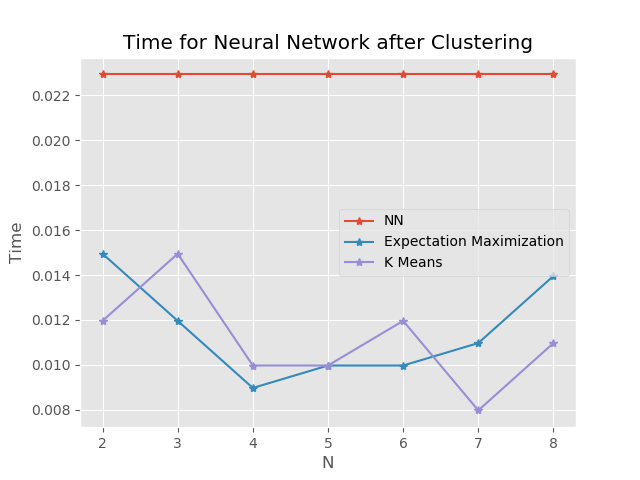
\includegraphics[width=1.2\linewidth]{../figures/wine_nn_cluster_time.png}
     \caption{Time}\label{Fig:wine_nn_cluster_time}
   \end{minipage}
\end{figure}

Fig.\ref{Fig:wine_nn_cluster} shows the accuracy of neural networks trained by data that is preprocessed by different clustering algorithms. Fig.\ref{Fig:wine_nn_cluster_time} shows the corresponding training time. The x-axis is different selection of N. From the figure, it is clear that the training time after using clustering algorithms is much shorter. For the accuracy, proper selection of number of clusters will produce a higher accuracy. I believe this is because clustering gives additional information for neural network. A good clustering means the data is being assigned some ``correct'' feature, so it takes less time to train and can get a better accuracy. On the other hand, a bad clustering will mislead the neural network by containing many data points which are actually belongs to multiple classes. Then the accuracy will drop, as the experiments show.
\end{document}
